\chapter{Исследовательская часть}

В данном разделе представлены результаты исследования, которое заключалось в нахождении
зависимости времени выполнения запроса с использованием индексов и без, а так же технические 
характеристики устройства, на котором данное исследование было сделано.

\section{Технические характеристики}

Исследование было выполнено на устройстве, 
которое имеет следующие характеристики:

\begin{itemize}
    \item операционная система macOS Sonoma 14.1.1 \cite{macos};
    \item 2 GHz 4-ядерный процессор Intel Core i5;
    \item оперативная память: 16 Гб.
\end{itemize}

\section{Исследование}

Для проведения исследования зависимости времени выполнения запроса при наличии индексов и без
был выбран поиск пользователя по почте.

Замеры производились при количестве записей от 10000 до 1000000 c шагом 10000. Для того, чтобы 
избежать статистические выбросы каждый замер происходил 1000 раз, качестве результата
бралось среднее значение, которое получалось делением суммы всех повторных замеров на их количество.

Результаты исследования представлены в таблице \ref{tab:res}.

\clearpage

\begin{table}[!ht]
    \centering
    \caption{\label{tab:res} Результаты замера времени выполнения запроса
    по почте в зависимости от использовани индексов, с и без.}
    \begin{tabular}{|l|l|l|}
    \hline
        Количество  & Время выполнения & Время выполнения\\
        зарегистрированных & запроса & запроса \\
        пользователей & (без индексов), мкс & (с индексами), мкс \\ \hline
        10 000 & 4 943 & 2 188 \\ \hline
        20 000 & 5 930 & 2 266 \\ \hline
        30 000 & 6 044 & 2 735 \\ \hline
        40 000 & 6 515 & 2 819 \\ \hline
        50 000 & 7 145 & 3 128 \\ \hline
        60 000 & 10 028 & 4 472 \\ \hline
        70 000 & 10 507 & 4 524 \\ \hline
        80 000 & 10 305 & 4 616 \\ \hline
        90 000 & 13 005 & 4 628 \\ \hline
        10 0000 & 14 542 & 4 827 \\ \hline
    \end{tabular}
\end{table}

По полученным данным был составлен график \ref{graph:res}.

\begin{figure}[H]
    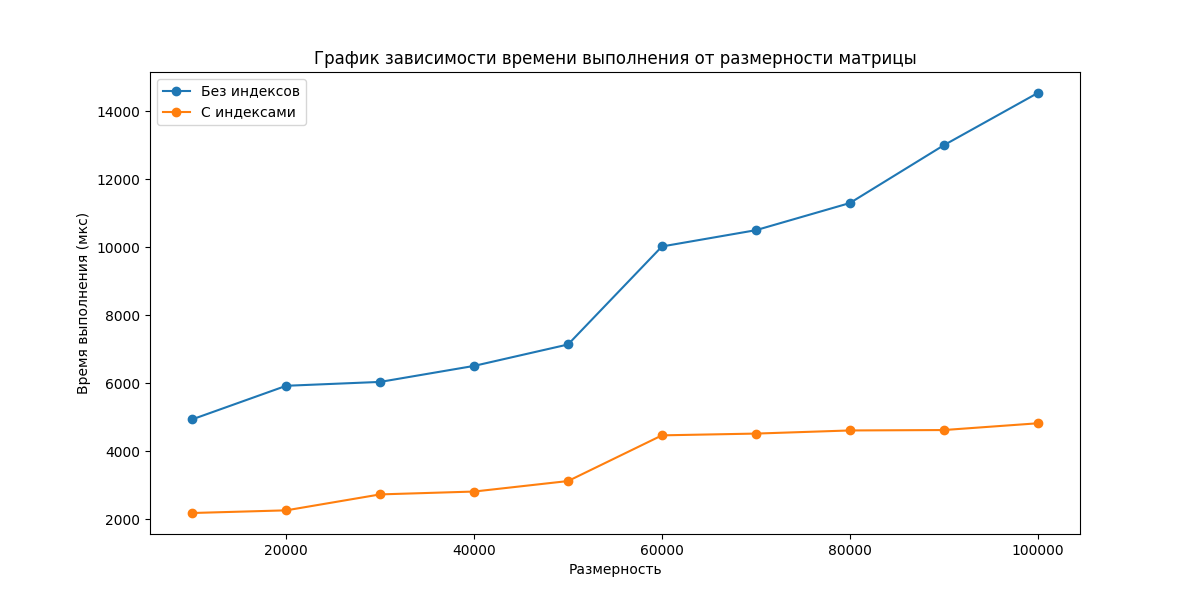
\includegraphics[width=1\linewidth]{img/graph.png}
    \caption{\label{graph:res} График зависимости времени выполнения запроса
    по почте в зависимости от использования индексов, с и без, и количества записей }
\end{figure}
\noindent

По результатам исследования можно сделать вывод 
о том, что использование индекса помогает ускорить
время запроса примерно в 2-3 раза.

\section*{Вывод}

В данном разделе было описано и проведено исследование, которое
заключалось в получении зависимости выполнения запроса
с использлванием индексов и без. Так же были описаны технические 
характеристики устройства, на котором проводилось 
исследование. 

Результом исследования стал вывод о том, что использование индексов помогает ускорить
время выполнения запроса в 2-3 раза.
